In order to explore and measure the comparative merits that are to be
enjoyed by the employment of a RON, any experiments must be carried out in
a network that resembles a realistic environment, particularly with respect
to the routing processes that take place within the network. To that end,
the Emulab environment~\cite{Emulab} was chosen as the setting in which
experimental network topologies would be developed, in lieu of access to an
actual live network.

Two main design goals were set regarding the emulated network topology: It
should
\begin{inparaenum}[(a)]
\item \label{req:scalable}
  be easily scalable, extensible and customisable in order to facilitate
  experimentation for a broad range of applications, not limited to our
  specific case; and
\item \label{req:bgp}
  rely on BGP to enable inter-AS routing. 
\end{inparaenum}
The latter goal can be thought as being relevant to the former one, since
the primary functions of BGP is to facilitate scalability, but its main
purpose is to ensure that the network behaves in a realistic way, slow
convergence issues due to link outings, security issues, etc.\ included.

Consequently, one is led to install and configure software routers on the
nodes of the emulated topology, since the preset routing schemes that can
be defined through the Emulab \texttt{ns} syntax cannot support the
flexibility of the desired behaviour. This, in conjunction with the
aforementioned goal \cref{req:scalable}, defines another design goal: The
network configuration must be done \emph{automatically}---otherwise, the
emulated network topology would scarcely serve as a convenient
experimentation tool, particularly as the size of the network increases.

To meet these three requirements, we developed a \emph{multi-AS network
  generator}. The generator is provided as a bundle of \texttt{.ns},
\texttt{AWK} and \texttt{C-shell} scripts that perform the generation,
configuration and initialisation of the desired emulated network. All
relevant code can be found at
\url{https://github.com/ailiop/cps214/tree/master/code/multi-as}.


\subsection{The network generator}
\label{sec:netgen}

The functionality of our network generator can be considered, roughly, to
address two issues:
\begin{inparaenum}[(a)]
\item the network topology and
\item routing within the network.
\end{inparaenum}

\paragraph{Topology}

Using the network topology generator, we are able to easily instantiate a
class of multi-AS network topologies. These topologies adhere to the
following specification: Each AS is comprised by a full mesh of routers and
a number of LANs; each LAN, in turn, is comprised by a number of terminal
(e.g.\ PC) nodes which share a single router as gateway. The inter-AS links
must be explicitly set by the user, the reasoning being that one would not
expect too many inter-AS connections to be defined in an experimental
emulated network. The creation of an inter-AS link can be flagged in a
\texttt{.txt} file, simply by specifying the two routers that will be
linked by way of the ASNs and serial numbers within their respective
ASes. It should also be noted that, although the intra-AS links are set to
form a full mesh, a user may easily obtain custom topologies by explicitly
removing any unwanted links, either by modifying the \texttt{.ns} script
(e.g.\ by including a source file that deletes a number of links) or by
dynamically killing the links after the network is
instantiated.\footnote{It should be noted that the latter approach should
  not be preferred as it would result in allocation of redundant nodes in
  the Emulab testbed.}

The topology can be scaled through a few parameters in the \texttt{.ns}
script that control the number and size of ASes in the network, as well as
the number and size of LANs within each AS. Additional parameters control
the configuration (e.g.\ delay and bandwidth) of the inter-AS, intra-AS and
LAN links, as well as a number of other elements of the network
configuration.

Technically, the size of the network is limited to $8$ routers and as many
LANs per AS, $253$ terminals per LAN, $256$ ASes, and $16384$ inter-AS
connections, while it is easy to modify the network creation script to
balance between the number of allowed ASes and that of routers (and LANs)
per AS. However, much tighter limits will likely be imposed on the actual
experiment by the testbed environment.

\paragraph{Routing}

After the network topology has been created and instantiated in Emulab,
routing must be set up. To that end, we make use of the \emph{Quagga}
software routing suite,\footnote{\url{http://www.nongnu.org/quagga/}} and
enable BGP routing over OSPF.

The routing configuration process is commenced as soon as a node is booted
in the Emulab experiment. The first step is to link the kernel's interfaces
(e.g.\ \texttt{eth3}) to the corresponding IP addresses (e.g.\
\texttt{192.168.0.3/30}); this cannot be done in advance, since the
assignment of IP addresses to interfaces is random in the Emulab
environment.\footnote{The Emulab \emph{control link} is an exception in
  that it is always attached to \texttt{eth0}. Furthermore, Emulab does
  provide a way to statically specify the interfaces of links, but this
  functionality is problematic and it greatly limits the nodes that can be
  used.}

Then, configuration files for the relevant Quagga daemons\footnote{Three
  daemons are needed: \texttt{zebra}, \texttt{ospfd} and \texttt{bgpd}.}
are generated. The OSPF process is configured to assign a router's links to
areas (currently all links are assigned to area $0$) and to retrieve
\emph{connected} and BGP routes, giving higher precedence to the connected
ones. The BGP process is configured to retrieve the OSPF routes and to set
up BGP peering between the node and its immediate neighbours. The next step
is, of course, to invoke the routing daemons and wait for convergence.

As far as the terminal nodes (i.e.\ the ones that form the various LANs,
sans the respective gateways) are concerned, these need not be running
routing software, as they will only act as sinks from the perspective of
the OSPF/BPG routing processes. Hence, the set of IP prefixes that are
associated with the emulated network are simply added to its default
routing table with the corresponding LAN gateway router as the next hop.

It should be noted that, while router nodes must be booted with a Linux OS
image that contains the Quagga package,\footnote{A ready option in the
  Emulab of the University of Utah is the custom image we created:
  \href{https://www.emulab.net/showosinfo.php3?osid=3042}{\texttt{UBUNTU11-64-QUAGGA}}.}
the terminal nodes may be booted with any Linux or Free-BSD image. This
will likely allow for running most application-layer experiments with
minimal configuration. A possible scenario would be for one to develop an
experiment script that is supposed to run on the terminal nodes and simply
have it be invoked from within \texttt{startup-pc.csh}.

Lastly, since experimentation is an iterative process and manually
resetting the network to its initial state (perhaps after reconfiguring the
routing, too) would be even more tedious than re-initiating the Emulab
experiment, a script is provided that crawls among all nodes in the network
and completely resets the node initialisation process.


\subsection{The dark side of Emulab}
\label{sec:emulab-problems}

Emulab has proved to provide a great environment for network emulation in a
realistic way. Unfortunately, ``realistic'' also implies that a host of
things might go wrong. Here we mention an error that might occur while
swapping a large experiment in Emulab which would cause the network to
exhibit aberrant routing behaviour, as its source might be hard to track
down.

\Cref{fig:link-errors} shows the Emulab Linktest log for an experiment that
uses 36 nodes. It can be seen that a link appears to exhibit a very high
packet loss rate and another one seems to be completely dead. However, that
is not the case: Links that appear to be dead after running Linktest may
still allow a packet to go through from time to time (e.g.\ once every one
or two minutes); depending on the placement of such links in a topology,
this could cause the BGP routes to be constantly changing.

\begin{figure}
  \centering
  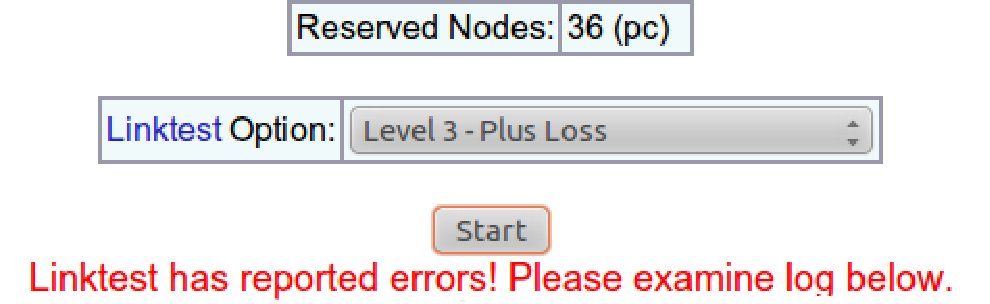
\includegraphics[width=0.4\linewidth]{link-errors-1}
  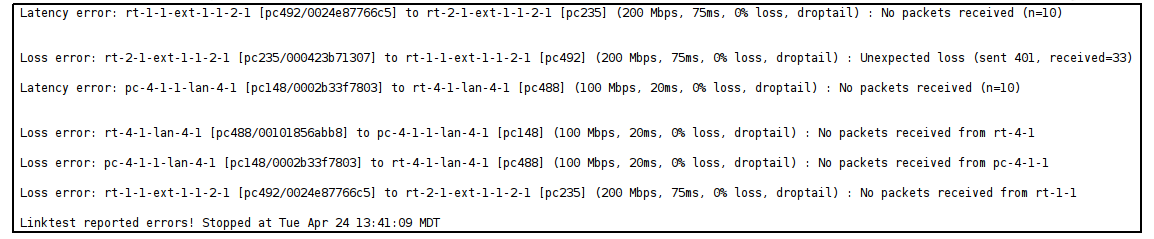
\includegraphics[width=\linewidth]{link-errors-2}
  \caption{Emulab Linktest log for an experiment of $36$ nodes. The link
    \texttt{ext-1-1-2-1} seems to exhibit a very high packet loss rate,
    whereas the link \texttt{lan-4-1} appears to be dead.}
  \label{fig:link-errors}
\end{figure}


\subsection{An example network}
\label{sec:network-example}

\Cref{fig:big-net} shows a visual representation of a network topology with
eight ASes, generated with our network generator script. It should be
evident that the automatic routing configuration procedure is invaluable to
facilitating experimentation with such large topologies. The figure was
obtained using the Emulab visualisation tool.

\begin{figure}[!b]
  \centering
  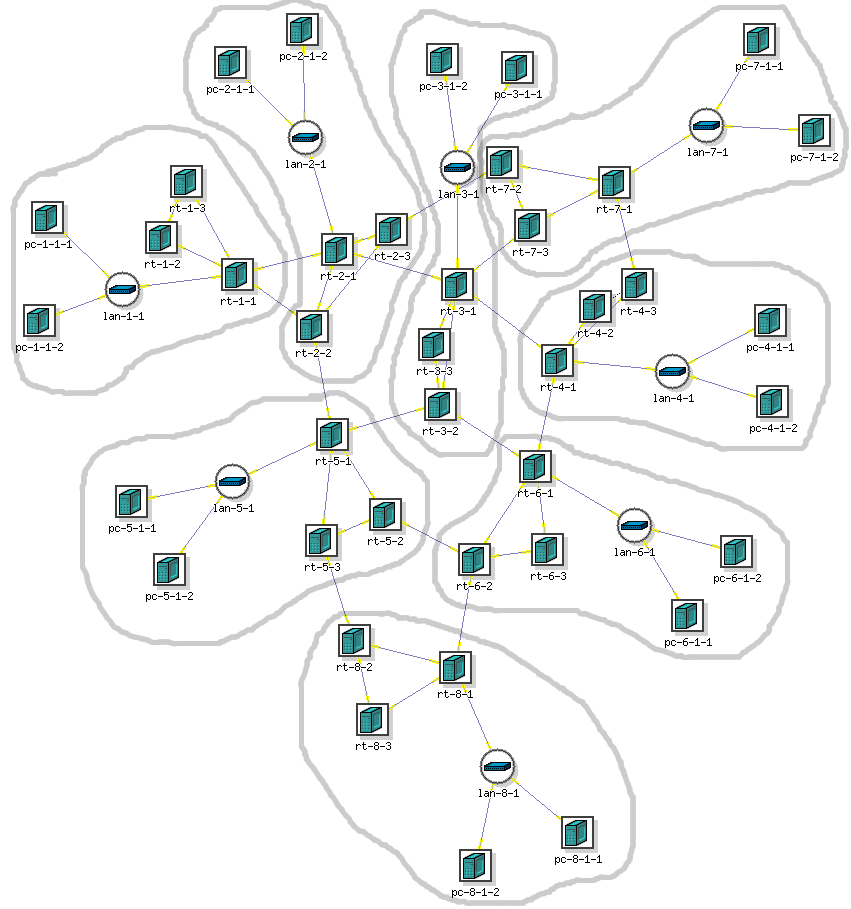
\includegraphics[width=\linewidth]{big-net}
  \caption{A network topology of 8 ASes, with 3 router nodes and 2 terminal
    nodes each. The gray borders delimit individual ASes.}
  \label{fig:big-net}
%  \vspace*{8pt}
\end{figure}


%%% Local Variables: 
%%% mode: latex
%%% TeX-master: "project-cps214"
%%% End: 

%  LocalWords:  Emulab LANs ASNs intra BGP OSPF Quagga Linktest ASes
